%% ------------------------------------------------------------------------- %%
\chapter{Construção do processo}
\label{cap:construcao}

%% ------------------------------------------------------------------------- %%
\section{Definições}
\label{sec:definicoes}

Tomemos $\Nz = \{ 1, 2, 3, \ldots\}$ A esse conjunto adicionaremos um
novo símbolo, que denotaremos por $\infty$. Chamaremos esse novo
conjunto de $\Nzb$.

O processo K será um processo estocástico em tempo contínuo, cujo
espaço de estados será $\Nzb$. Chamaremos os elementos de $\Nzb$ de
estados ou sítios do processo.

Como parâmetros do processo, teremos duas famílias de números reais
estritamente positivos, $\gamma_x$ e $\lambda_x$, $x \in \Nz$. Além de
uma constante $c \in [0, \infty)$.  Para um estado $x \in \Nz$,
podemos interpretar $\gamma_x$ como o tempo médio para o processo sair
de $x$ e $\lambda_x$ vai controlar a taxa com que o processo tende a
entrar em $x$. Enquanto que $c$ controla o tempo em que o estado fica
em $\infty$.

Seguindo \cite{fontes:08}, iremos definir o processo K através de uma
construção. O espaço de probabilidade, $\Omega$, onde iremos defini-lo
será um espaço que admita as seguintes famílias de variáveis
aleatórias independentes:

\begin{itemize}
\item $\{ N_x: x \in \Nz \}$: processos pontuais de Poisson
  independentes, onde $N_x$ tem taxa $\lambda_x$ para cada $x \in \N$.
\item $\{T_n^x: x \in \Nzb , \, n = 0, 1, 2, 3, \ldots \}$: variáveis
  aleatórias exponencias de média $1$.
\end{itemize}

Para $t \geq 0$, iremos denotar por $N_x(t)$ o número de marcas do
processo de poisson $N_x$ no intervalo $[0, t]$, marcas essas que
iremos denotar por $0 < \sigma_1^x < \sigma_2^x < \ldots$ .

Agora podemos definir uma função aleatória que será nossa principal
ferramenta para trabalhar com esse processo. Para $t \geq 0$ e $y \in
\Nzb$, sob a convenção que $\gamma_\infty = 0$:

\begin{equation}
  \label{def:Gamma}
  \Gamma(t) = \Gamma^y_c (t) = \gamma_y T_0^y
  + \sum_{x \in \N} \sum_{n = 1}^{N_x(t)}
  \gamma_x T_n^x
  + ct
\end{equation}

Por convenção, considere que $\sum_{i=1}^{0}( \bullet ) = 0$.

Agora vamos impor duas restrições nos nossos parâmetros. Que serão:
\begin{align}
  \sum_{x \in \Nz} \lambda_x\gamma_x < +\infty\\
  \sum_{x \in \Nz} \lambda_x = \infty.
\end{align}

A primeira fará com que $\Gamma$ seja \qc finita para todo $t \in
\R^+$, enquanto que o segundo fará com que o conjunto $\{\sigma^x_i: x
\in \Nz, \, i \geq 1\}$ seja denso em $\R$. Veremos na Seção
\ref{sec:visualizacao} que o processo K sem essa segunda condição é
bastante simples.

Chamaremos o processo K iniciado em $y \in \Nb$ de $X^y_c$. Ele é
definido, para $t \geq 0$, da seguinte forma:

\begin{equation}
  \label{def:procK}
  X(t) = X^y_c (t) =
  \begin{cases}
    y, & \textrm{ se }  t < \gamma_y T_0^y\\
    x, & \textrm{ se } \Gamma^y_c(\sigma_i^x-) \leq t <
    \Gamma^y_c(\sigma^x_i)
    \textrm{ para algum } i \\
    \infty, & \textrm{ caso contrário.}
  \end{cases}
\end{equation}

Note que para que essa definição faça sentido, temos que o limite a
esquerda $\Gamma (\sigma_i^x-)$ deve existir. Isso será estabelecido
na Proposição \ref{prop:gamma-cadlag}.

Quando puder ficar subentendido, nós vamos omitir a condição inicial
e/ou o parâmetro $c$ das notações.

Note que essa construção nos dá um acoplamento de processos K com
parâmetros $(\lambda_x, \gamma_x)_{x \in \Nz}$ para toda condição
inicial $y$ e todo $c \geq 0$. Isso será muito útil para mostrar
alguns resultados.



\section{Visualização}
\label{sec:visualizacao}

Para essa seção, vamos supor que $\sum_{x \in \Nz} \lambda_x <
\infty$. Nesse caso a sobreposição de todos os processos de Poisson
$\{N_x : x \in \Nz\}$ será um processo de Poisson de taxa $\sum_{x \in
  \Nz} \lambda_x$. Assim podemos $\qc$ enumerar as marcas desse
processo, denotando-as por $ \sigma_1 < \sigma_2 < \ldots$.

O gráfico da função $\Gamma^y$, fora das marcas $\sigma_1, \sigma_2,
\ldots$ se comporta como é uma reta de inclinação $c$, e nas marcas
essa função tem dá saltos, de tamanho $\gamma_x T^x_i$, para algum $x$
e algum $i$. A figura \ref{fig:graf_gamma} ilustra uma possível
realização de $\Gamma^y$.


Pela nossa construção, esses saltos corresponderão ao tempo que o
processso passa nos estados de $\Nz$, enquanto que no resto do tempo
ele está no $\infty$.

Assim nosso processo K se reduzirá a um processo Markoviano de
saltos.

No caso $c > 0$, iniciando em um estado $y$, o processo permanece
nesse estado um tempo exponencial de média $\gamma_y$. Passado esse
tempo ele pula para o $\infty$, onde permanece um tempo exponencial de
média $\frac{c}{\sum_{x \in \Nz} \lambda_x}$, escolhendo um novo
estado $y$ com probabilidade $\frac{\lambda_y}{\sum_{x \in \Nz}
  \lambda_x}$.

No caso $c=0$, nós permanecemos em cada estado $x$ um tempo
exponencial de média $\gamma_x$, e escolhemos pular para um novo estado $y$
com probabilidade $\frac{\lambda_y}{\sum_{x \in \Nz} \lambda_x}$.
Note que nesse caso nós nunca visitamos o $\infty$, vale até mesmo que
$X^\infty(0) \neq \infty$ \qc.


\begin{figure}
  \centering
  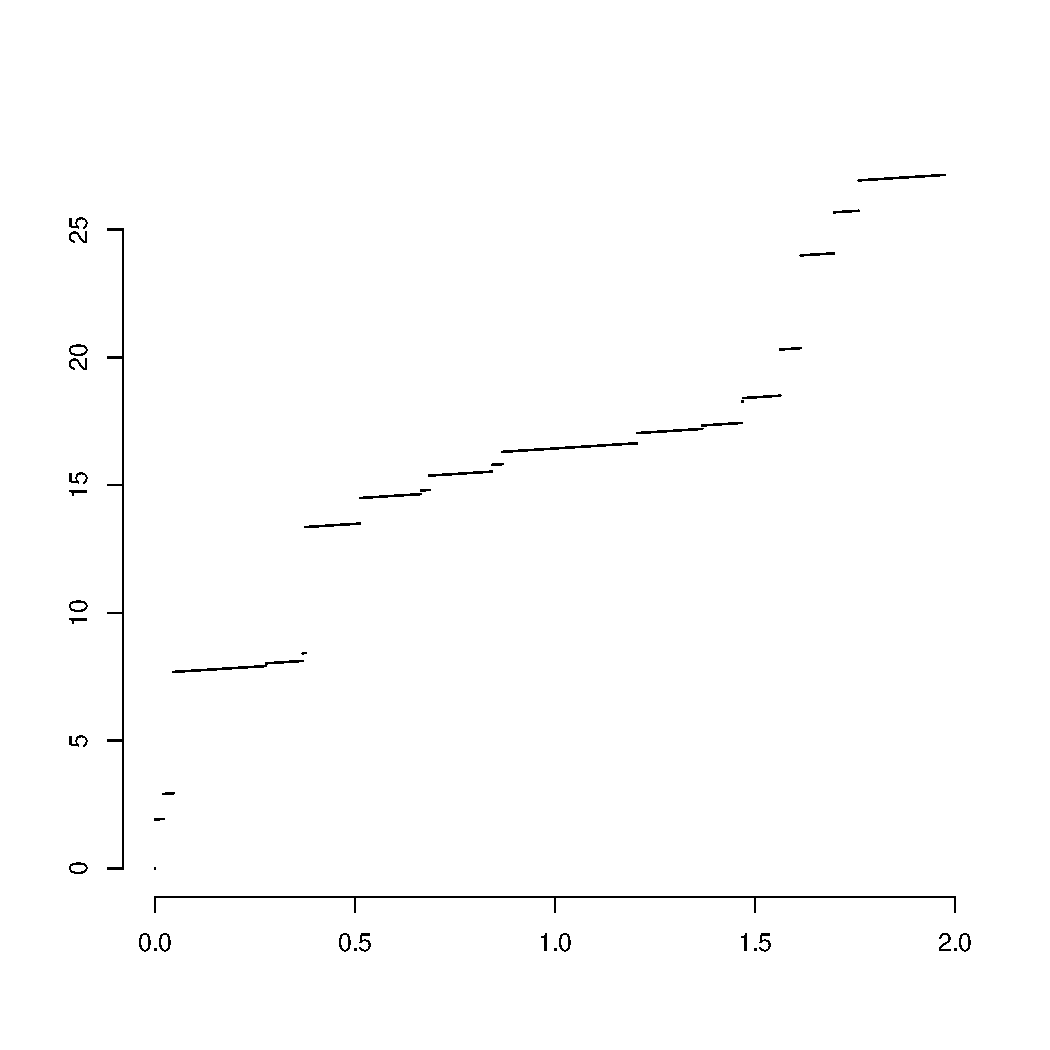
\includegraphics[width=.80\textwidth]{graf_gamma}
  \caption{Um exemplo de realização de $\Gamma$ quando $\sum_{x \in
      \Nz} \lambda_x < \infty$}
  \label{fig:graf_gamma}
\end{figure}

\section{Topologia sobre o espaço de estados}
\label{sec:topologia}

Será útil para alguns resultados munirmos $\Nzb$ de uma
topologia. Para isso considere a seguinte métrica:
\begin{equation}
  \label{eq:metrica}
  d(x, y) = \left\lvert \frac{1}{x} - \frac{1}{y} \right\rvert,
\end{equation}
para $x, y \in \Nzb$, sob a convenção de que $\frac{1}{\infty} = 0$.

Essa métrica induz uma topologia bastante natural, onde todos os
pontos $x \in \Nz$ são pontos isolados, e uma sequência converge ao
$\infty$ nessa topologia se ela divergir para infinito da maneira
usual.

Uma função $f: \Nzb \to \R$ será contínua se e somente se
$f(\infty) = \lim_{x \to \infty} f(x)$.

Vale ainda que essa topologia é compacta, nos dando boas propriedades
para trabalhar.

%%% Local Variables: 
%%% TeX-master: "tese"
%%% End: 
